% =============================================================================
% Lecture 02: ARIMA, VAR & Multivariate Models
% ECON 8310: Business Forecasting
% University of Nebraska at Omaha
% =============================================================================

\documentclass[aspectratio=169, 11pt]{beamer}

\input{header}

% ---- Lecture metadata --------------------------------------------------------
\title[ARIMA, VAR \& Multivariate]{ARIMA, VAR \& Multivariate Models}
\subtitle{ECON 8310: Business Forecasting --- Lecture 2}
\author{Department of Economics}
\institute{University of Nebraska at Omaha}

% =============================================================================
\begin{document}
% =============================================================================

\begin{frame}
  \titlepage
\end{frame}

% ---- Outline ----------------------------------------------------------------
\begin{frame}{Lecture Outline}
  \tableofcontents
\end{frame}

% =============================================================================
\section{Stationarity and Differencing}
% =============================================================================

\sectionslide{Stationarity and Differencing}{%
  Before fitting any model, the series must have a stable mean and variance.}

% --- Slide: Weak stationarity -------------------------------------------------
% Figure: scripts/figures/lecture02_figures.py (stationarity_band); ADF as in Lab 2.
\begin{frame}{What Is Stationarity?}
  \begin{columns}[c]
    \begin{column}{0.47\textwidth}
      \begin{definitionbox}{Weak (Covariance) Stationarity}
        $\{y_t\}$ is \textbf{weakly stationary} if:
        \begin{enumerate}\small\itemsep1pt
          \item constant mean: $\E[y_t] = \mu$
          \item constant variance: $\Var(y_t) = \sigma^2 < \infty$
          \item $\Cov(y_t, y_{t-k}) = \gamma_k$ depends only on lag $k$, not on $t$
        \end{enumerate}
      \end{definitionbox}
      {\small Conditions 1--2, pictured: the series stays inside a \textbf{horizontal band
      of fixed width}. TX\_1 HOUSEHOLD fails; its weekly change passes.}
    \end{column}
    \begin{column}{0.51\textwidth}
      \centering
      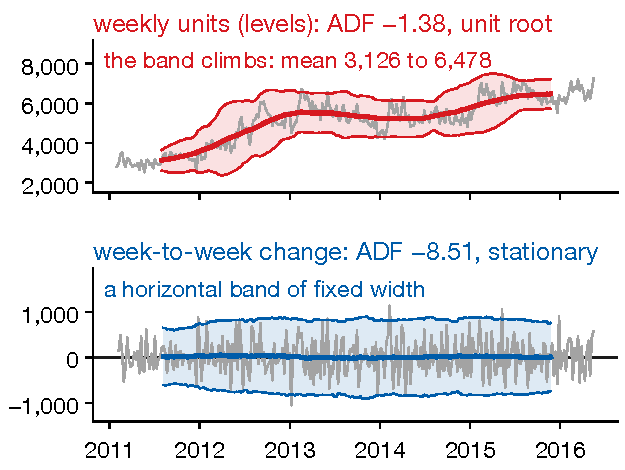
\includegraphics[height=5.1cm]{../Figures/Lecture02_ARIMA_VAR/stationarity_band.pdf}
    \end{column}
  \end{columns}
  \vspace{0.1cm}
  {\small A drifting mean leaves no single value to forecast; a growing variance widens
  intervals without bound. Differencing removes a stochastic trend; a log stabilizes the
  variance.}
\end{frame}

% --- Slide: Unit root + differencing ------------------------------------------
\begin{frame}{Unit Roots and Differencing}
  \textbf{AR(1):} $y_t = \phi_1\,y_{t-1} + \varepsilon_t$. Give it one unit shock and watch
  what is left of it:
  \begin{center}
    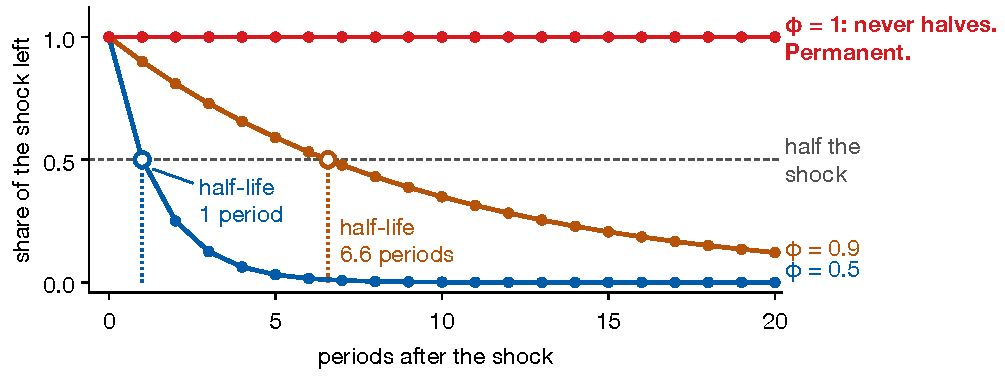
\includegraphics[height=3.9cm]{../Figures/Lecture02_ARIMA_VAR/shock_response.pdf}
  \end{center}
  \vspace{-0.3cm}
  Below one, each period keeps the same share $\phi_1$, so the shock halves every
  $\ln 0.5 / \ln \phi_1$ periods. At $\phi_1 = 1$, a \textbf{unit root}, it never fades: a
  random walk. \textbf{Differencing}, $\Delta y_t = y_t - y_{t-1}$, removes it. $d$ counts
  first differences; $D$ counts seasonal ones, $\Delta_{12}y_t = y_t - y_{t-12}$.
\end{frame}

% --- Slide: Testing ------------------------------------------------------------
\begin{frame}{Testing for a Unit Root}
  Rule of thumb: a visible trend or growing variance means the series is likely
  non-stationary. Then test formally.

  \vspace{0.15cm}
  \textbf{ADF} ($H_0$: unit root) and \textbf{KPSS} ($H_0$: stationary) test
  \emph{opposite} nulls, so run both, and be suspicious when they disagree.
  \begin{warningbox}
    \textbf{Do not over-difference.} Differencing an already-stationary series induces
    negative autocorrelation that you then have to model away. Difference, re-test, and stop
    at $d = 1$ once the result is stationary.
  \end{warningbox}
  \muted{\footnotesize Lecture 1's TX\_1 HOUSEHOLD: ADF $-1.38$ on the levels (a unit root),
  $-8.51$ after one difference (stationary). So $d = 1$.}
\end{frame}

% --- Slide: Spurious regression ----------------------------------------------
\begin{frame}{Why the Rule Exists: Spurious Regression}
  Differencing is not bookkeeping. Skip it and the statistics actively lie to you.
  \begin{center}
  \begin{tikzpicture}[scale=0.92, every node/.style={scale=0.92}]
    \draw[->, unoblack] (0,0) -- (8.2,0) node[right, font=\scriptsize]{$t$};
    \draw[unoblack] (0,-0.3) -- (0,2.5);
      \draw[unocrimson, line width=1.1pt] (0.00,0.05) -- (0.20,0.17) -- (0.39,0.13) -- (0.58,0.23) -- (0.78,0.43) -- (0.98,0.54) -- (1.17,0.85) -- (1.36,0.74) -- (1.56,0.79) -- (1.76,0.72) -- (1.95,0.63) -- (2.15,0.64) -- (2.34,0.72) -- (2.54,0.83) -- (2.73,0.96) -- (2.93,1.38) -- (3.12,1.56) -- (3.31,1.34) -- (3.51,1.41) -- (3.71,1.35) -- (3.90,1.31) -- (4.09,1.57) -- (4.29,1.57) -- (4.49,1.29) -- (4.68,1.38) -- (4.88,1.37) -- (5.07,1.22) -- (5.27,1.11) -- (5.46,1.04) -- (5.66,1.08) -- (5.85,1.05) -- (6.04,1.10) -- (6.24,1.45) -- (6.44,1.36) -- (6.63,1.27) -- (6.83,1.27) -- (7.02,1.50) -- (7.21,1.42) -- (7.41,1.70) -- (7.61,1.52);
      \draw[unoblack, line width=1.1pt] (0.00,0.12) -- (0.20,-0.15) -- (0.39,-0.25) -- (0.58,-0.20) -- (0.78,0.08) -- (0.98,0.11) -- (1.17,-0.13) -- (1.36,-0.05) -- (1.56,-0.22) -- (1.76,0.02) -- (1.95,0.01) -- (2.15,0.34) -- (2.34,0.36) -- (2.54,0.22) -- (2.73,0.00) -- (2.93,-0.03) -- (3.12,0.08) -- (3.31,0.32) -- (3.51,0.39) -- (3.71,0.30) -- (3.90,0.42) -- (4.09,0.21) -- (4.29,0.33) -- (4.49,0.24) -- (4.68,0.52) -- (4.88,0.72) -- (5.07,0.81) -- (5.27,0.68) -- (5.46,0.80) -- (5.66,0.90) -- (5.85,0.84) -- (6.04,0.77) -- (6.24,1.01) -- (6.44,0.98) -- (6.63,1.08) -- (6.83,1.35) -- (7.02,1.13) -- (7.21,1.47) -- (7.41,1.67) -- (7.61,1.60);
    \node[unocrimson, font=\scriptsize, right] at (7.7,2.05) {$x$};
    \node[unoblack,   font=\scriptsize, right] at (7.7,1.35) {$y$};
  \end{tikzpicture}
  \end{center}
  \vspace{-0.25cm}
  Two independent random walks --- \textbf{no shared cause, no relationship at all}. Their
  \emph{changes} correlate at $-0.13$, which is the truth. But their
  \emph{levels} correlate at +0.62, and that is what OLS sees.
  \begin{warningbox}
    \small \textcite{GrangerNewbold1974} showed this rejects ``no relationship'' about
    \textbf{three-quarters} of the time at the 5\% level. The regression is not finding a
    relationship --- it is finding that both series wander. \textbf{Difference first.}
  \end{warningbox}
\end{frame}

% --- Slide: ACF and PACF for identification -----------------------------------
\begin{frame}{ACF and PACF: Model Identification}
  The \textbf{autocorrelation function}, $\rho_k = \mathrm{Corr}(y_t, y_{t-k})$, measures
  how $y_t$ relates to its own past. The \textbf{partial} autocorrelation controls for the
  lags in between, which separates a direct effect from one inherited through them.

  \vspace{0.2cm}
  Read together, they identify the model:
  \begin{center}
    {\small
    \begin{tabular}{lll}
      \toprule
      \textbf{Model} & \textbf{ACF} & \textbf{PACF} \\
      \midrule
      AR($p$)   & Tails off geometrically & \pos{Cuts off} after lag $p$ \\
      MA($q$)   & \pos{Cuts off} after lag $q$ & Tails off geometrically \\
      ARMA      & Tails off & Tails off \\
      RW / I(1) & Decays slowly & Big spike at lag 1 \\
      \bottomrule
    \end{tabular}
    }
  \end{center}
\end{frame}

% --- Slide: What ACF/PACF actually look like ---------------------------------
% Figure: scripts/figures/lecture02_figures.py (acf_theory), exact values from ArmaProcess.
\begin{frame}{What Those Patterns Actually Look Like}
  \begin{center}
    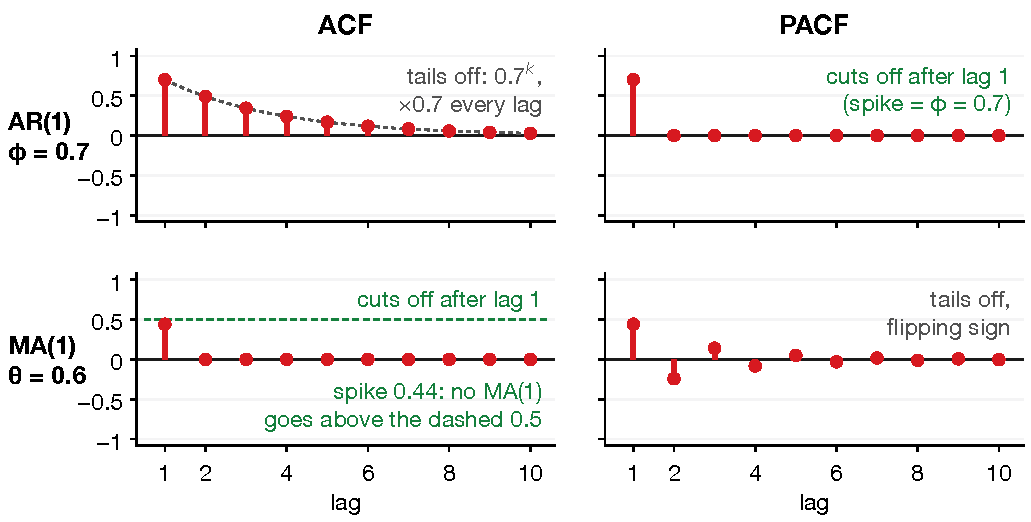
\includegraphics[height=5.6cm]{../Figures/Lecture02_ARIMA_VAR/acf_theory.pdf}
  \end{center}
  \vspace{-0.3cm}
  Exact values, not a sample. Read the pair: the \pos{sharp cut-off} gives the order, the
  \emph{slow decay} says which side it is on. The AR(1) ACF is a staircase: each lag keeps
  $\phi$ of the one before.
\end{frame}

% --- Slide: a real series, before and after differencing ---------------------
% Figure: scripts/figures/lecture02_figures.py (acf_levels_vs_diff). TX_1, not CA_1: Lab 2 has
% students read CA_1 HOUSEHOLD's ACF themselves.
\begin{frame}{Difference First, Then Read the ACF}
  Lecture 1's TX\_1 HOUSEHOLD series, before and after one difference:
  \begin{center}
    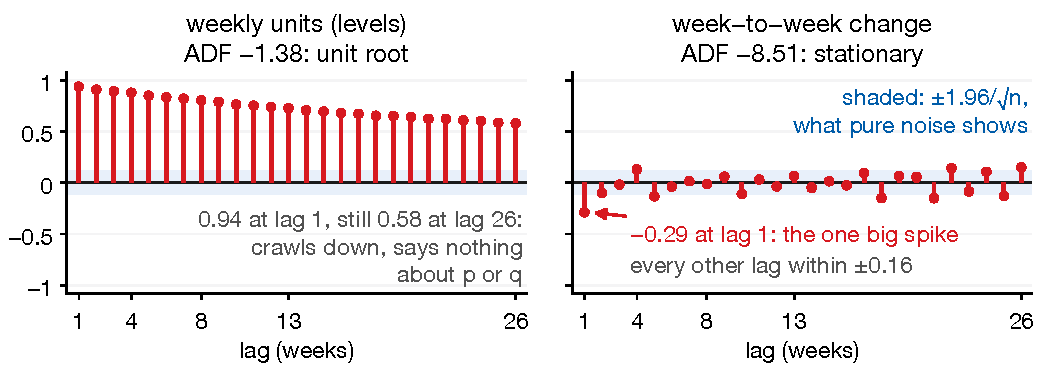
\includegraphics[height=3.9cm]{../Figures/Lecture02_ARIMA_VAR/acf_levels_vs_diff.pdf}
  \end{center}
  \vspace{-0.3cm}
  The levels' ACF crawls down whatever the process is: it only says you have not differenced
  yet. The change has one negative spike at lag 1, the MA(1) signature. So ARIMA(0,1,1),
  which is simple exponential smoothing: Lecture 1's $\alpha = 0.62$ implies $\rho_1 = -0.33$;
  the data show $-0.29$.
\end{frame}

% =============================================================================
\section{ARIMA Models}
% =============================================================================

\sectionslide{ARIMA Models}{%
  Combine differencing with AR and MA components into one unified model.}

% --- Slide: ARIMA definition --------------------------------------------------
\begin{frame}{ARIMA($p$,$d$,$q$)}
  \begin{definitionbox}{ARIMA($p$,$d$,$q$) Model}
    {\small Difference the series $d$ times, $y'_t = \Delta^d y_t$, then fit an ARMA($p$,$q$)
    to $y'_t$:}
    \vspace{-4pt}
    \[
      y'_t = c + \sum_{i=1}^{p}\phi_i\, y'_{t-i} + \varepsilon_t + \sum_{j=1}^{q}\theta_j\,\varepsilon_{t-j}
    \]
    \vspace{-8pt}
  \end{definitionbox}
  Familiar models are corners of this space: \textbf{ARIMA(0,1,0)} is a random walk,
  \textbf{ARIMA(1,0,0)} an AR(1), and \textbf{ARIMA(0,1,1)} simple exponential smoothing.

  \vspace{0.1cm}
  \textbf{A forecast by hand.} ARIMA(1,1,0) with $\hat{\phi}_1 = 0.5$, $y_{100} = 120$ and
  $y_{99} = 118$. The last change was 2, so the next is half of it:
  $\hat{y}_{101|100} = 120 + 0.5 \times 2 = \mathbf{121}$.

  \vspace{0.1cm}
  \muted{\footnotesize \textbf{Python:} \texttt{pmdarima.auto\_arima()} searches orders;
  \texttt{statsmodels.SARIMAX} fits the order you choose.}
\end{frame}

% --- Slide: SARIMA ------------------------------------------------------------
% Figure: scripts/figures/lecture02_figures.py (sarima_acf). CA_1 FOODS daily, the only daily series.
\begin{frame}{SARIMA: Adding Seasonal Terms}
  Seasonal data also correlate at lags $m, 2m, 3m, \ldots$, and SARIMA adds AR and MA terms
  there: \textbf{two ARIMA models at different time scales}, $(p,d,q)$ for the short run and
  $(P,D,Q)[m]$ for the season.
  \begin{center}
    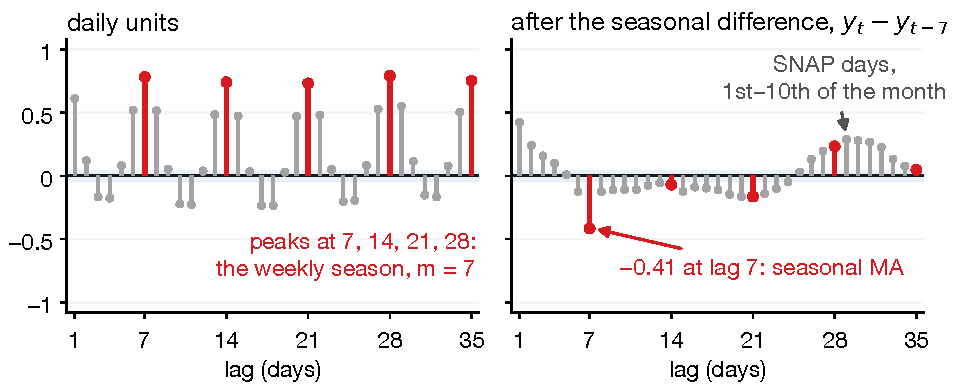
\includegraphics[height=4.25cm]{../Figures/Lecture02_ARIMA_VAR/sarima_acf.pdf}
  \end{center}
  \vspace{-0.3cm}
  {\small CA\_1 FOODS is daily, so $m = 7$ here (monthly data use $m = 12$). One seasonal
  difference, $D = 1$, removes the peaks; the spike left at lag 7 points to one seasonal MA
  term, $Q = 1$.}
\end{frame}

% --- Slide: SARIMA workflow ----------------------------------------------------
\begin{frame}{SARIMA in Practice: A Four-Step Workflow}
  \textbf{Practical workflow:}
  \begin{enumerate}\itemsep4pt
    \item ADF / KPSS $\to$ choose $d$
    \item Seasonal unit root test $\to$ choose $D$
    \item ACF / PACF on the differenced series $\to$ guide $p, q, P, Q$
    \item Minimize AIC, then check the residual ACF with a Ljung-Box test
  \end{enumerate}
  \vspace{0.3cm}
  \textbf{Ljung-Box} ($H_0$: the residuals are white noise) is the one people skip. Here a
  \emph{large} $p$-value is the good outcome: nothing left to model.

  \vspace{0.2cm}
  \muted{\small Monthly retail: start from SARIMA(1,1,1)(0,1,1)[12] and make anything
  fancier beat it.}
\end{frame}

% =============================================================================
\section{VAR Models}
% =============================================================================

\sectionslide{VAR Models}{%
  When two series influence each other, model them together symmetrically.}

% --- Slide: Why multivariate --------------------------------------------------
\begin{frame}{Why Use Multiple Series?}
  Every model so far --- ETS, ARIMA --- uses only $y_t$'s own history. But business
  variables are linked: consumer sentiment today moves retail spending next month, and
  advertising moves sales over the following weeks.
  \begin{keybox}
    If $x_t$ carries information about $y_{t+h}$ that is not already in $y_t$'s own history,
    including $x_t$ reduces forecast error.
  \end{keybox}
  \textbf{Granger causality} \parencite{Granger1969} is the formal test of exactly that
  claim. It comes right after the VAR.
\end{frame}

% --- Slide: VAR or ARIMAX ------------------------------------------------------
\begin{frame}{VAR or ARIMAX: Which Way Does Influence Run?}
  The modeling choice turns on whether the influence runs one way or both:

  \vspace{0.2cm}
  \begin{columns}[T]
    \begin{column}{0.48\textwidth}
      \textbf{VAR --- symmetric}
      \begin{itemize}\small\itemsep0pt
        \item Every variable predicts every other
        \item Use when influence runs both ways
        \item No variable is privileged
        \item Example: retail sales and unemployment (the lab)
      \end{itemize}
    \end{column}
    \begin{column}{0.48\textwidth}
      \textbf{ARIMAX --- one direction}
      \begin{itemize}\small\itemsep0pt
        \item $x_t$ drives $y_t$, not the reverse
        \item Use when the causal story is clear
        \item Needs a forecast of $x_t$ itself
        \item Example: advertising $\to$ sales
      \end{itemize}
    \end{column}
  \end{columns}
\end{frame}

% --- Slide: VAR(1) definition -------------------------------------------------
\begin{frame}{The VAR($p$) Model}
  For two stationary series, each equation regresses on the lags of \emph{both}:
  \[
    \begin{cases}
      y_{1t} = c_1 + a_{11}\,y_{1,t-1} + a_{12}\,y_{2,t-1} + \varepsilon_{1t}\\[2pt]
      y_{2t} = c_2 + a_{21}\,y_{1,t-1} + a_{22}\,y_{2,t-1} + \varepsilon_{2t}
    \end{cases}
  \]
  The cross terms carry the value: $a_{12}$ is how much $y_{2,t-1}$ predicts $y_{1t}$,
  exactly what a univariate AR throws away. If $a_{12} = a_{21} = 0$, the system is two
  separate ARs.
  \begin{warningbox}
    \textbf{Parameter explosion.} $k$ variables and $p$ lags make $k^2 p$ coefficients: at
    $k=5$, $p=4$, \textbf{100}, often more than a monthly series has observations. Keep
    $k \leq 4$, or use a LASSO-VAR.
  \end{warningbox}
  \muted{\footnotesize \textbf{Python:}
  \texttt{statsmodels.tsa.api.VAR}; \texttt{var.fit(maxlags=p, ic='bic')} picks $p$ by BIC.}
\end{frame}

% --- Slide: Granger causality -------------------------------------------------
\begin{frame}{Granger Causality Test}
  \begin{definitionbox}{Granger Causality}
    $x_t$ \textbf{Granger-causes} $y_t$ if past values of $x_t$ help predict $y_t$
    \emph{beyond what $y_t$'s own past already explains}.
  \end{definitionbox}
  \textbf{The test:} fit the $y$-equation with and without the $x$-lags; an $F$-test of
  $H_0$: all $x$-lag coefficients are zero.

  \vspace{0.2cm}
  \textbf{Not structural causality.} It tests predictive content: a rooster reliably predicts
  sunrise. Say ``predictive of,'' never ``causes.''
\end{frame}

% --- Slide: Granger on the lab's macro data -----------------------------------
% Figure: scripts/figures/lecture02_figures.py (granger_covid); Lab 2 Step 6's numbers. The
% pre-2020 cut is a lab exercise, so it is not shown.
\begin{frame}{Granger on Real Data: The COVID Window}
  \textbf{Does unemployment Granger-cause retail sales?} Lab 2's monthly FRED data:
  \begin{center}
    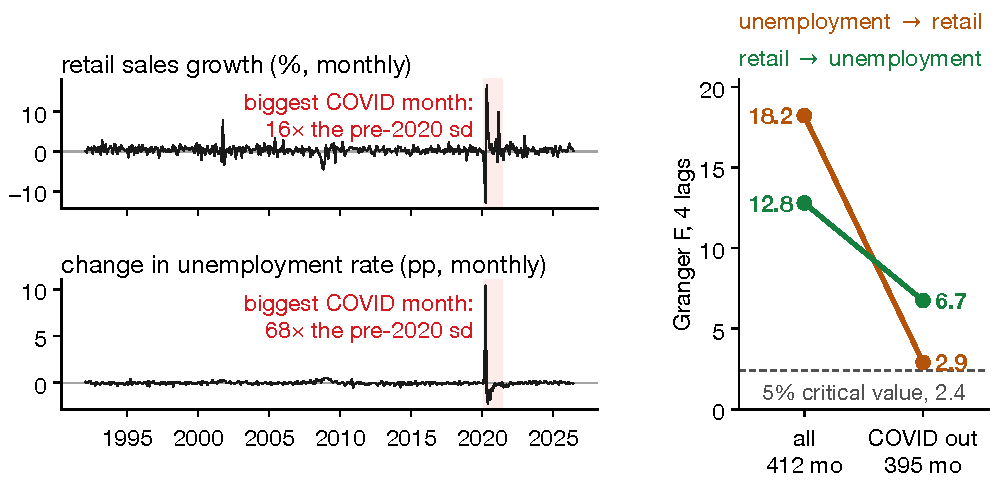
\includegraphics[height=5.0cm]{../Figures/Lecture02_ARIMA_VAR/granger_covid.pdf}
  \end{center}
  \vspace{-0.35cm}
  {\small Both directions are significant in both samples; one shock decides which looks
  stronger. With COVID: unemployment $\to$ retail. Without its 17 months: retail $\to$
  unemployment.}
\end{frame}

% --- Slide: ARIMAX -----------------------------------------------------------
\begin{frame}{ARIMAX: Exogenous Variables with ARIMA Errors}
  When one variable clearly \emph{drives} another, use ARIMAX.
  \begin{definitionbox}{ARIMAX Model}
    \[
      y_t = \mathbf{x}_t'\boldsymbol{\beta} + \eta_t,
      \qquad \eta_t \sim \mathrm{ARIMA}(p,d,q)
    \]
    $\mathbf{x}_t$ are exogenous regressors; $\eta_t$ absorbs the autocorrelation left in
    the residuals.
  \end{definitionbox}
  \textbf{Use it when} the direction is clear (advertising $\to$ sales), you have $x_t$ or
  can forecast it, and adding it cuts cross-validated error. Check that last one.

  \vspace{0.15cm}
  \textbf{The catch:} forecasting $y_{t+h}$ needs $x_{t+h}$, a forecast of your own
  predictor. Without one, use a VAR, which forecasts every series it contains.

  \vspace{0.1cm}
  \muted{\footnotesize \textbf{Python:} \texttt{SARIMAX(y, exog=X, order=(p,d,q)).fit()}}
\end{frame}

% =============================================================================
\section{Key Takeaways and Roadmap}
% =============================================================================

\sectionslide{Key Takeaways and Roadmap}{%
  Stationarity, ARIMA, VAR, and ARIMAX form the classical time series toolkit.}

% --- Slide: Key Takeaways -----------------------------------------------
\begin{frame}{Key Takeaways}
  \begin{keybox}
    {\small
    \begin{enumerate}
      \item \textbf{Stationarity first:} test with ADF and KPSS (opposite nulls); difference
            away a unit root.
      \item \textbf{ACF} gives the MA order, \textbf{PACF} the AR order --- read after
            differencing.
      \item \textbf{ARIMA($p$,$d$,$q$)} is an ARMA on the differenced series; SARIMA adds
            seasonal terms; \texttt{auto\_arima} searches.
      \item \textbf{VAR} treats series symmetrically; keep $k \leq 4$. \textbf{Granger} tests
            predictive content, not causation.
      \item \textbf{ARIMAX} adds exogenous predictors, if you can forecast them.
    \end{enumerate}
    }
  \end{keybox}
  \muted{\itshape Next: Generalized Additive Models (GAMs) ---
  flexible, interpretable nonlinear forecasting with Prophet and pyGAM.}
\end{frame}

% --- References ---------------------------------------------------------------
\begin{frame}[allowframebreaks]{References}
  \printbibliography[heading=none]
\end{frame}

% =============================================================================
\end{document}
% =============================================================================
